\documentclass[11pt]{article}
\usepackage[margin=1in]{geometry}
\usepackage{graphicx}
\usepackage{booktabs}
\usepackage{amsmath}
\usepackage{hyperref}
\usepackage{multirow}
\usepackage[numbers]{natbib}

\title{DietConv Revisited:\\Memory-Efficient Strip-Buffered GEMM Convolution with a Tiled v2 Schedule}
\author{Shiva Deviah}
\date{\today}

\begin{document}
\maketitle

\begin{abstract}
We revisit DietConv, a strip-buffered alternative to full \texttt{im2col} lowering for convolution. The original DietConv schedule preserves the GEMM-friendly structure of lowered convolution while replacing the global lowered matrix with a per-output-row strip buffer. We then present DietConv-v2, a practical refinement that tiles the output width, reuses row windows across adjacent output rows, and autotunes tile width. Across a CPU-only evaluation spanning NumPy, C++, and a compiled PyTorch extension, the clearest result is reduced temporary state and lower measured process-memory deltas than explicit \texttt{im2col} or \texttt{unfold}, with frequent wins over native framework convolution on memory as well. Runtime results are more shape-dependent: DietConv-v2 is often competitive and sometimes faster than the baseline strip-buffer implementation, but it is not a universal replacement for mature native kernels. We argue that DietConv is best understood as a family of memory-efficient lowering schedules rather than a single monolithic kernel.
\end{abstract}

\section{Introduction}
Convolution implementations often trade memory for matrix-multiply reuse. Explicit lowering, as popularized by frameworks such as Caffe \citep{jia2014caffe}, converts convolution into GEMM by materializing overlapping input patches into a large matrix. This strategy is effective for throughput but duplicates data aggressively. DietConv was originally conceived as a compromise: preserve the GEMM decomposition while replacing the full lowered matrix with a narrow strip buffer that covers only one output row at a time.

This paper has two goals. First, it documents the original DietConv idea as a reproducible algorithmic object rather than an unpublished poster concept. Second, it introduces DietConv-v2, a practical refinement that tiles the output width, reuses intermediate row windows, and adds autotuning. Our claim is not that DietConv-v2 universally beats native convolution in mature frameworks such as PyTorch \citep{paszke2019pytorch}. Instead, we argue that DietConv is a publishable concept because it offers a distinct and useful point in the space between direct convolution and full explicit lowering: it reduces memory duplication structurally and can remain runtime-competitive in important CPU inference regimes.

The strongest result in this repository is memory behavior. Relative to explicit \texttt{im2col}/\texttt{unfold}, both DietConv variants dramatically reduce temporary state. The more practical question is how close a systems-aware implementation can get to native kernels while preserving that memory profile. DietConv-v2 is our answer to that question.

Our contributions are straightforward:
\begin{itemize}
    \item we document the original DietConv schedule clearly enough to reproduce and benchmark,
    \item we introduce DietConv-v2 as a tiled, autotuned refinement of the same strip-buffer idea,
    \item we provide an end-to-end artifact with NumPy, C++, and compiled PyTorch implementations, plus both explicit-workspace and sampled process-memory measurements.
\end{itemize}

\section{Background and Motivation}
The appeal of explicit lowering is simple: convolution becomes matrix multiplication. If the input tensor is rearranged into a matrix of sliding patches and the convolution kernels are flattened into rows, the forward pass can be computed with a single GEMM. This idea is especially attractive on CPUs because vendor BLAS libraries already provide highly tuned GEMM kernels.

The cost is duplication. Overlapping receptive fields are copied repeatedly into the lowered matrix, increasing both workspace and memory bandwidth pressure. In large-kernel or large-feature-map settings, the temporary matrix can be substantially larger than the working set actually needed at any moment.

DietConv revisits this decomposition by asking a narrower question: how much of the lowered matrix is truly needed at once? The original answer is ``one output row.'' DietConv-v2 sharpens that answer further to ``one output-row tile.''

\section{DietConv v1}
DietConv-v1 keeps the mathematical structure of lowered convolution but changes the schedule:
\begin{enumerate}
    \item Copy an $F_h$-row strip of the padded input for one output row.
    \item Reorder weights by kernel column so each kernel-column slice forms a GEMM-ready matrix.
    \item Accumulate one GEMM per kernel column into the output row.
\end{enumerate}

If the conventional \texttt{im2col} workspace is
\[
C \cdot F_h \cdot F_w \cdot H_{out} \cdot W_{out},
\]
then the DietConv-v1 strip buffer is
\[
C \cdot F_h \cdot W_{in}^{(\mathrm{padded})}.
\]
The arithmetic count is unchanged; the difference is the shape and lifetime of the temporary state.

\section{DietConv v2}
DietConv-v2 keeps the core strip-buffer identity but narrows the active window from a full output row to an output-width tile. It adds four practical refinements:
\begin{itemize}
    \item tile the output width so only the necessary source span is packed,
    \item reuse packed row windows across adjacent output rows when stride allows overlap,
    \item feed GEMM directly from the packed tile for stride-1 cases,
    \item autotune tile width and prefer the smallest workspace within 5\% of the fastest measured candidate.
\end{itemize}

These changes make DietConv-v2 an implementation-oriented improvement rather than a new algorithmic family. The expected tradeoff is straightforward: smaller tiles reduce temporary state and can improve locality, but they also increase packing overhead and make performance more sensitive to the chosen tile width.

\begin{figure}[t]
    \centering
    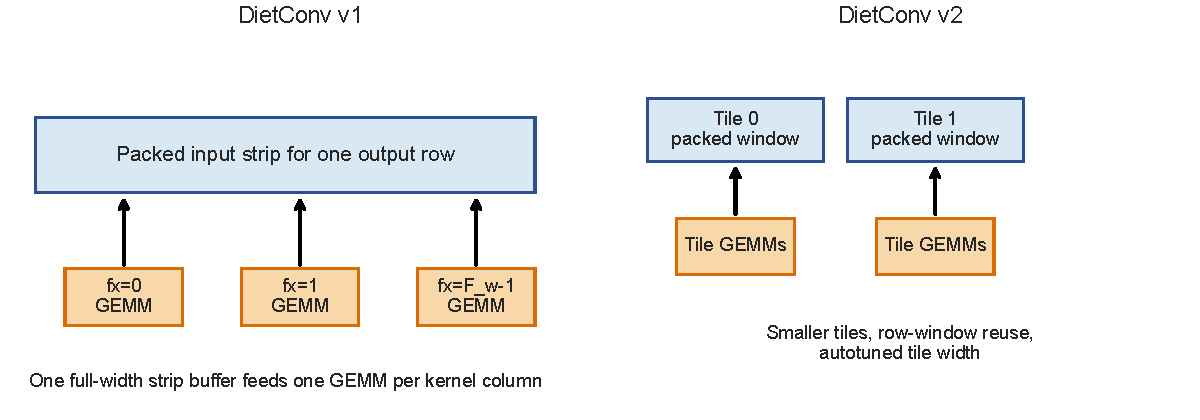
\includegraphics[width=\linewidth]{figures/dietconv_overview.pdf}
    \caption{Conceptual schedule difference between DietConv-v1 and DietConv-v2. Both preserve the per-kernel-column GEMM decomposition; v2 narrows the active lowering window and adds reuse across adjacent output rows.}
    \label{fig:overview}
\end{figure}

\section{Implementation}
We implement DietConv in three layers:
\begin{itemize}
    \item a NumPy reference implementation for clarity,
    \item a C++ CPU kernel using Accelerate GEMM for low-level timing,
    \item a compiled PyTorch CPU extension for framework-level comparisons.
\end{itemize}

The PyTorch path pre-packs weights, applies a small eligibility gate before using optimization-specific heuristics, and caches autotuned tile widths by shape and thread count. We also add an isolated-process memory benchmark so native PyTorch convolution can be compared using sampled peak RSS deltas rather than appearing as a fake zero-workspace baseline.

\section{Experimental Setup}
All reported results come from the repository artifact and are CPU-only. We report four classes of measurements:
\begin{itemize}
    \item NumPy reference benchmarks,
    \item C++ runtime and explicit workspace sweeps,
    \item compiled PyTorch runtime and explicit workspace sweeps,
    \item isolated-process PyTorch peak RSS deltas.
\end{itemize}

The evaluation emphasizes representative CNN-style layer shapes rather than end-to-end training. Numerical agreement is checked against either explicit \texttt{im2col} or native \texttt{conv2d}, and benchmark runs fail if the maximum absolute difference exceeds a fixed tolerance.

\section{Results}
\subsection{C++ Results}
The C++ path is the clearest view of the algorithm because it removes most Python overhead. Figure~\ref{fig:cpp-scaling} shows that DietConv-v2 often improves on DietConv-v1 in stride-1 size sweeps while preserving the expected workspace advantage over full \texttt{im2col}.

\begin{figure}[t]
    \centering
    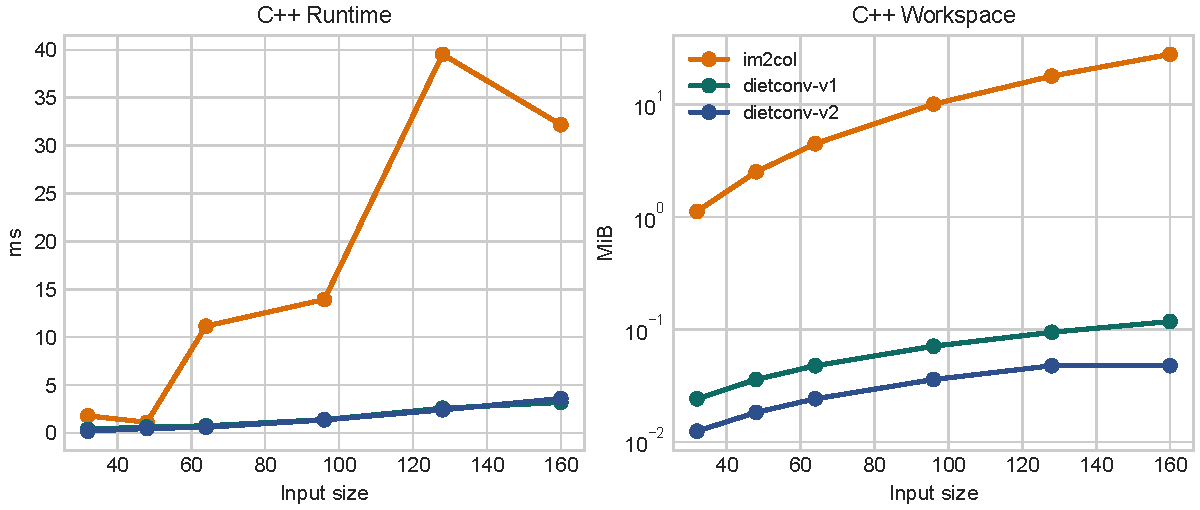
\includegraphics[width=\linewidth]{figures/cpp_size_scaling.pdf}
    \caption{C++ runtime and explicit workspace across the size sweep. DietConv-v2 is usually faster than DietConv-v1 on the tested stride-1 cases while remaining far smaller than full \texttt{im2col}.}
    \label{fig:cpp-scaling}
\end{figure}

\begin{table}[t]
\centering
\caption{Representative C++ runtime and explicit workspace results.}
\label{tab:cpp-runtime}
\begin{tabular}{lllll}
\toprule
Input & im2col & v1 & v2 & v2 ws (MiB) \\
\midrule
32 & 1.79 & 0.37 & 0.18 & 0.012 \\
48 & 1.11 & 0.62 & 0.46 & 0.018 \\
64 & 11.16 & 0.74 & 0.59 & 0.024 \\
96 & 13.93 & 1.39 & 1.36 & 0.036 \\
128 & 39.54 & 2.58 & 2.41 & 0.048 \\
160 & 32.18 & 3.19 & 3.59 & 0.048 \\
\bottomrule
\end{tabular}
\end{table}


\subsection{PyTorch Runtime Results}
The compiled PyTorch extension makes the framework comparison more realistic. Native \texttt{conv2d} remains a strong baseline, but DietConv-v2 is competitive with explicit \texttt{unfold} and often improves on DietConv-v1. The strongest interpretation is not universal runtime dominance; it is that a strip-buffered lowering schedule can stay practical after systems-aware implementation.

\begin{figure}[t]
    \centering
    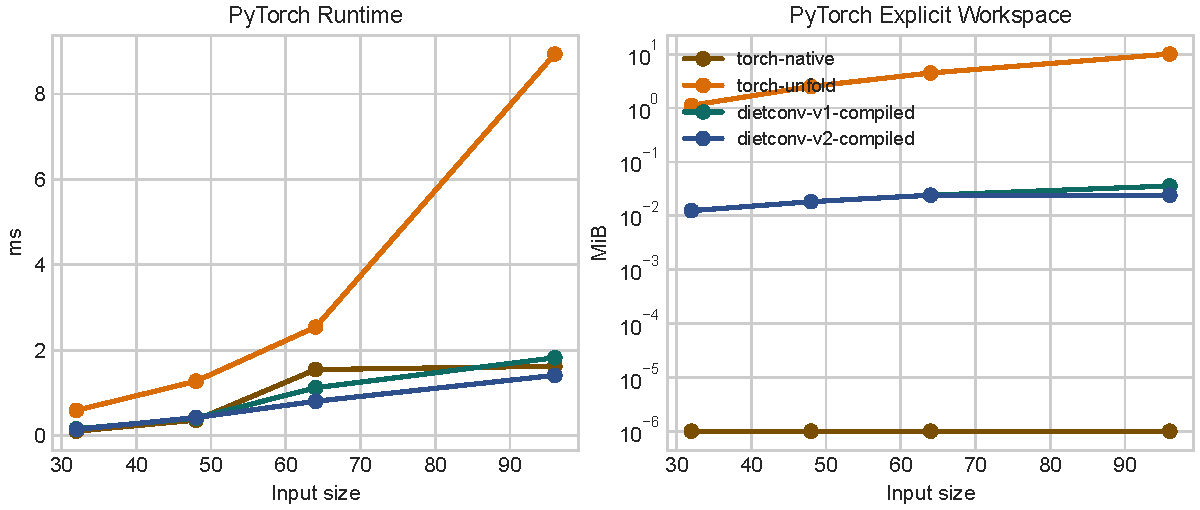
\includegraphics[width=\linewidth]{figures/torch_size_scaling.pdf}
    \caption{PyTorch runtime and explicit workspace. DietConv-v2 strongly reduces explicit lowering workspace and is competitive with the explicit \texttt{unfold} baseline.}
    \label{fig:torch-scaling}
\end{figure}

\begin{table}[t]
\centering
\caption{Representative PyTorch runtime results.}
\label{tab:torch-runtime}
\begin{tabular}{lllll}
\toprule
Input & native & unfold & v1 & v2 \\
\midrule
32 & 0.11 & 0.59 & 0.16 & 0.15 \\
48 & 0.37 & 1.28 & 0.41 & 0.42 \\
64 & 1.55 & 2.54 & 1.12 & 0.81 \\
96 & 1.63 & 8.93 & 1.82 & 1.41 \\
\bottomrule
\end{tabular}
\end{table}


\subsection{Measured Process Memory}
The most important addition beyond theoretical workspace is isolated-process RSS measurement. This changes the native-framework comparison materially: native PyTorch no longer appears to use zero memory. Figure~\ref{fig:torch-memory} and Table~\ref{tab:torch-memory} show that DietConv-v1 and DietConv-v2 often reduce measured process-memory deltas relative to both explicit \texttt{unfold} and native \texttt{conv2d}, though not uniformly.

\begin{figure}[t]
    \centering
    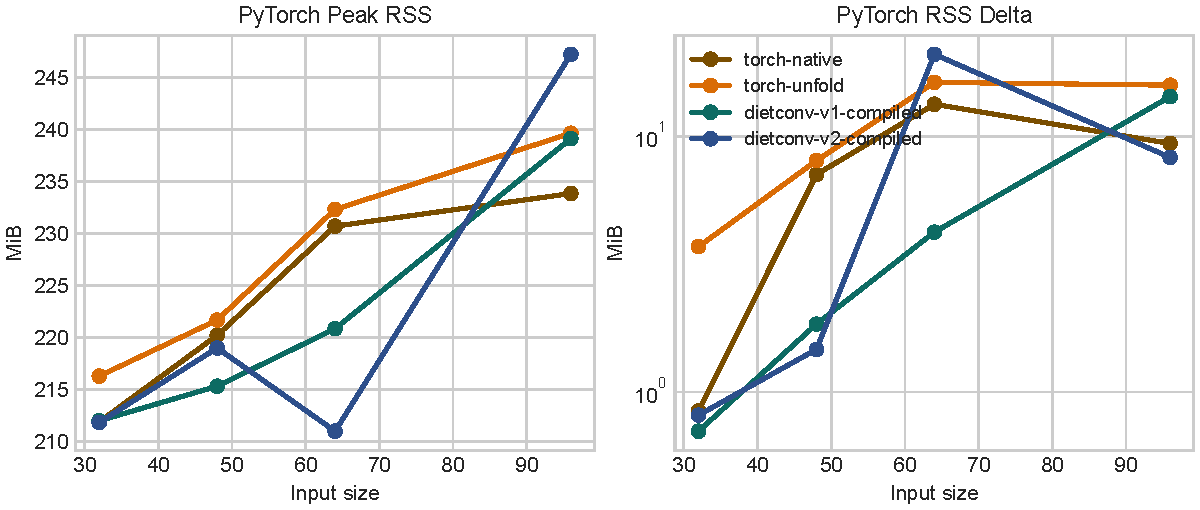
\includegraphics[width=\linewidth]{figures/torch_memory_scaling.pdf}
    \caption{PyTorch peak RSS and RSS delta across the size sweep, measured in isolated worker processes. The most consistent advantage of DietConv is memory behavior rather than universal runtime superiority.}
    \label{fig:torch-memory}
\end{figure}

\begin{table}[t]
\centering
\caption{Representative isolated-process RSS deltas for PyTorch backends.}
\label{tab:torch-memory}
\begin{tabular}{lllll}
\toprule
Input & native & unfold & v1 & v2 \\
\midrule
32 & 0.84 & 3.70 & 0.70 & 0.81 \\
48 & 7.09 & 8.03 & 1.84 & 1.47 \\
64 & 13.34 & 16.25 & 4.22 & 20.92 \\
96 & 9.38 & 15.84 & 14.30 & 8.27 \\
\bottomrule
\end{tabular}
\end{table}


\subsection{Ablation}
DietConv-v2 depends materially on tile width. Figure~\ref{fig:ablation} shows that the chosen tile width can move a case from clearly favorable to clearly unfavorable. This justifies the inclusion of autotuning and supports our framing of v2 as a practical schedule refinement rather than a parameter-free algorithm.

\begin{figure}[t]
    \centering
    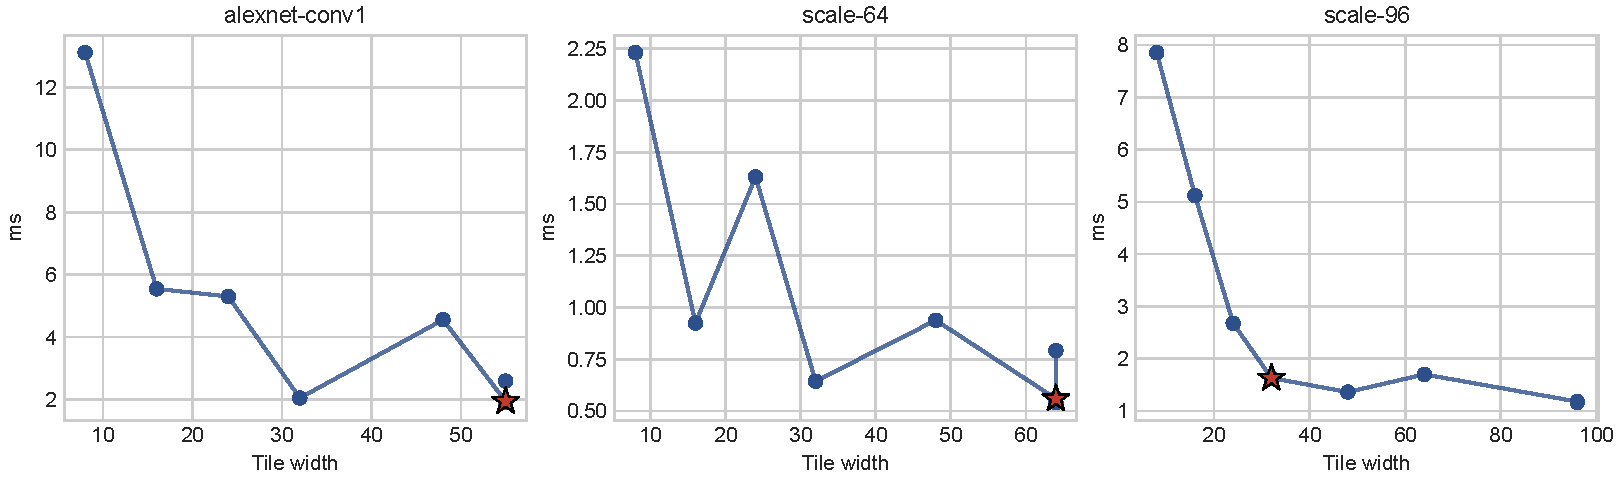
\includegraphics[width=\linewidth]{figures/v2_tile_ablation_cpp.pdf}
    \caption{DietConv-v2 tile-width ablation in the C++ path. The autotuned choice is highlighted in red. Tile width is a real performance knob, not a cosmetic implementation detail.}
    \label{fig:ablation}
\end{figure}

\section{Limitations}
This work is intentionally limited. The current artifact is CPU-only, focuses on inference-like single-batch settings, and measures process RSS rather than exact allocator-internal memory usage. DietConv-v2 also still exhibits bad cases, especially shapes where tiling overhead dominates or autotuned tile choices leave runtime on the table. The PyTorch extension is forward-only and does not attempt to replace framework-native kernels for training workloads. These limitations do not invalidate the concept, but they do constrain the strongest defensible claim: DietConv is a compelling memory-efficient lowering family, not yet a universally superior convolution backend.

\section{Conclusion}
DietConv is publishable as a concept when presented as a family of memory-efficient lowering schedules rather than as a universally superior convolution kernel. The original strip-buffered schedule remains compelling because it reduces duplication structurally. DietConv-v2 strengthens the practical case with tiling, row reuse, and autotuning, and the resulting implementation stack demonstrates that the idea can survive contact with modern systems code. The clearest contribution is not that DietConv-v2 always wins, but that memory-efficient GEMM-based convolution remains a meaningful design point worth documenting and studying.

\bibliographystyle{plainnat}
\bibliography{references}

\end{document}
